% assignment_7.tex - Assignment 7 for Data Fusion class (Fall 2014)
% Chanmann Lim - November 2014

\documentclass[a4paper]{article}

\usepackage[margin=1 in]{geometry}
\usepackage{amsmath}
\usepackage{listings}
\usepackage{graphicx}

\everymath{\displaystyle}

\begin{document}
\title{CS 8790: Report for assignment 7}
\author{Chanmann Lim}
\date{November 10, 2014}
\maketitle

\subsection*{Report:} ~\\
\indent The state of a target moving with constant velocity in 2D coordinate is observed. A sequence of the 2D measurements come with the corresponding \emph{timestamp}, at which each observation was taken, the mean $(x, y)$ and the upper triangular elements of the square root of the covariance $sqrtm(R)$ thus observation is now in the form of $(t\_z, z, R)$. \\

One way to start is to initialize our filter with time zero, zero mean and velocity and infinite covariance. \\
\begin{align*}
t = 0, 
x = \begin{bmatrix}
		0 \\ 0 \\ 0 \\ 0
	\end{bmatrix}, 
P = \begin{bmatrix}
		100000000 & 0 & 0 & 0 \\
		0 & 100000000 & 0 & 0 \\
		0 & 0 & 100000000 & 0 \\
		0 & 0 & 0 & 100000000
	\end{bmatrix}
\end{align*} \\
\noindent Yet, combining the estimate and the observation is not feasible unless both measurements are valid at the same \emph{timestamp} which leads to the prediction of the state of the estimate to the same timestamp as the observation using constant velocity model $F$. \\
\begin{align*}
F \quad (x, P) \to (Fx, FPF')
\end{align*} \\
, where
\begin{align*}
F = \begin{bmatrix}
		1 & 0 & \Delta{t} & 0 \\
		0 & 1 & 0 & \Delta{t} \\
		0 & 0 & 0 & 0 \\
		0 & 0 & 0 & 0
	\end{bmatrix}
\end{align*} \\

\noindent And since the observation comes in lower dimensionality (without velocity) than the state estimate we have to use transformation matrix $H$ to project down the state estimate before combining them using innovation fusion equation. \\
\begin{align*}
H = \begin{bmatrix}
		1 & 0 & 0 & 0 \\
		0 & 1 & 0 & 0 
	\end{bmatrix}
\end{align*} \\

\paragraph{1.1 } The state of the target at the time of the final observation is : \\
\begin{align*}
\text{mean with standard deviation} = 
	\left(\begin{matrix}
		245.277904 & ,   &    0.002747 \\
    	510.449761 & ,   &    0.001239 \\
      	0.280005 & ,     &  0.000007 \\
      	0.600000 & ,     &  0.000002 \\
	\end{matrix}\right)
\end{align*}
\begin{align*}
x\_final = \begin{bmatrix}
		245.277904 \\
    	510.449761 \\
      	0.280005 \\
      	0.600000 
	\end{bmatrix}
\end{align*}
\begin{align*}
P\_final = \begin{bmatrix}
		0.00000754  &  -0.00000074   &  0.00000002  &  -0.00000000  \\
   		-0.00000074  &   0.00000153  &  -0.00000000  &   0.00000000 \\
    	0.00000002  &  -0.00000000  &   0.00000000  &  -0.00000000 \\
   		-0.00000000  &   0.00000000  &  -0.00000000  &   0.00000000 
	\end{bmatrix}
\end{align*} \\

\paragraph{1.2 } The prediction of the state of the target one hour after the time of the final observation $(t=927.969649836)$ : \\
\begin{align*}
x(4527.969650) = \begin{bmatrix}
		1253.296210 \\
   		2670.451308 \\
      	0.280005 \\
      	0.600000  
	\end{bmatrix}
\end{align*}
\begin{align*}
P(4527.969650) =  \begin{bmatrix}
		    0.00082509  &  -0.00013653  &   0.00000021  &  -0.00000003 \\
   			-0.00013653  &   0.00008861  &  -0.00000004  &   0.00000002 \\
    		0.00000021  &  -0.00000004   &  0.00000000  &  -0.00000000 \\
   			-0.00000003  &   0.00000002  &  -0.00000000   &  0.00000000
	\end{bmatrix}
\end{align*} \\

\paragraph{1.3 } The plots of the sequence of normalized x and y innovations separately : \\
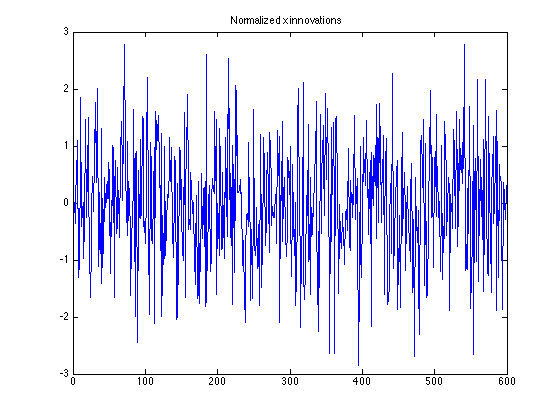
\includegraphics[scale=.4]{target_1_x_inno.png}
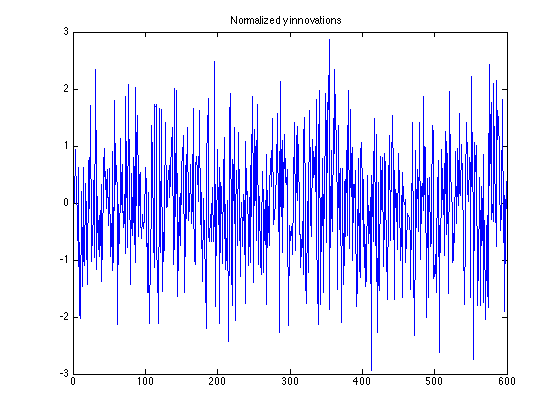
\includegraphics[scale=.4]{target_1_y_inno.png} \\

The normalized x innovations is obtained by $(z - Hx)(1)/\sqrt{S(1,1)}$ and y innovations = $(z - Hx)(2)/\sqrt{S(2,2)}$, where $S(1,1)$ and $S(2,2)$ is the diagonal values of the innovation covariance.\\

\paragraph{1.4 } The Percentage of x and y innovations that are less than 0 is $[ 48.50\%, 49.00\% ]$ \\

The plot of the running percentage of the x and y innovations that are less than zero : \\
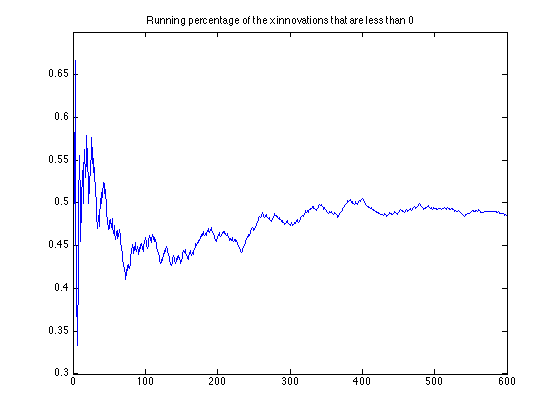
\includegraphics[scale=.4]{target_1_x_running.png}
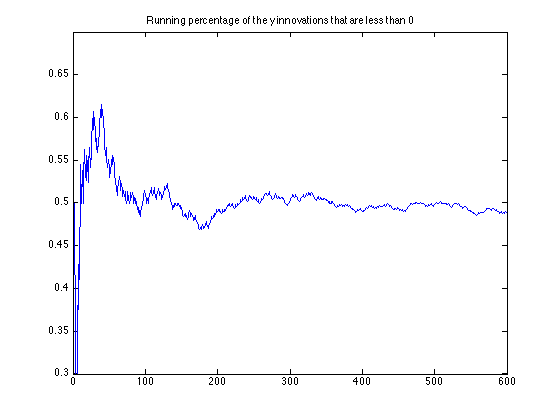
\includegraphics[scale=.4]{target_1_y_running.png} \\

For the second dataset, \texttt{Target2.txt}, the motion of the target deviates slightly from true constant velocity and the uncertainty should be increased to account for the deviation and this can be accomplished by incorporating the process noise covariance matrix $Q$ into P after applying the kinematic model $F$ previously used when predicting the state estimate into the future. \\
\begin{align*}
F \quad (x, P) \to (Fx, FPF' + Q)
\end{align*} \\
, where
\begin{align*}
Q = q \begin{bmatrix}
			1 & 0 & 0 & 0 \\
			0 & 1 & 0 & 0 \\
			0 & 0 & 0 & 0 \\
			0 & 0 & 0 & 0 \\
		\end{bmatrix} \Delta{t}
\end{align*} \\

The assumption here is that $Q$ is a reasonable process noise covariance matrix with respect to $\Delta{t}$ and $q$ and by empirically adjusting $q$ we can make the covariance big enough to cover the uncertainty produced during the course of tracking. \\

\paragraph{2.1 } \texttt{Target2.txt} without $q$ or $q=0$ : \\

\paragraph{2.1.1 } The state of the target at the time of the final observation is : \\
\begin{align*}
\text{mean with standard deviation} = 
	\left(\begin{matrix}
		-441.409777 & ,   &    0.002918 \\
    	249.803315 & ,   &    0.009243 \\
     	-0.495934 & ,   &    0.000006 \\
      	0.280004 & ,   &    0.000019
	\end{matrix}\right)
\end{align*}
\begin{align*}
x\_final = \begin{bmatrix}
		-441.409777 \\
    	249.803315 \\
     	-0.495934 \\
      	0.280004 
	\end{bmatrix}
\end{align*}
\begin{align*}
P\_final = \begin{bmatrix}
		0.00000852  &  -0.00000810  &   0.00000002  &  -0.00000002 \\
   -0.00000810  &   0.00008543  &  -0.00000002  &   0.00000017 \\
    0.00000002  &  -0.00000002  &   0.00000000  &  -0.00000000 \\
   -0.00000002  &   0.00000017  &  -0.00000000  &   0.00000000 
	\end{bmatrix}
\end{align*} \\

\paragraph{2.1.2 } The prediction of the state of the target one hour after the time of the final observation $(t=947.164131767)$ : \\
\begin{align*}
x(4547.164132) = \begin{bmatrix}
		  	-2226.770580 \\
   			1257.817758 \\
     		-0.495934 \\
      		0.280004 
	\end{bmatrix}
\end{align*}
\begin{align*}
P(4547.164132) = \begin{bmatrix}
    0.00063468  &  -0.00058346  &   0.00000016  &  -0.00000014 \\
   -0.00058346  &   0.00611027  &  -0.00000014  &   0.00000151 \\
    0.00000016  &  -0.00000014  &   0.00000000  &  -0.00000000 \\
   -0.00000014  &   0.00000151  &  -0.00000000  &   0.00000000
	\end{bmatrix}
\end{align*} \\

\paragraph{2.1.3 } The plots of the sequence of normalized x and y innovations separately : \\
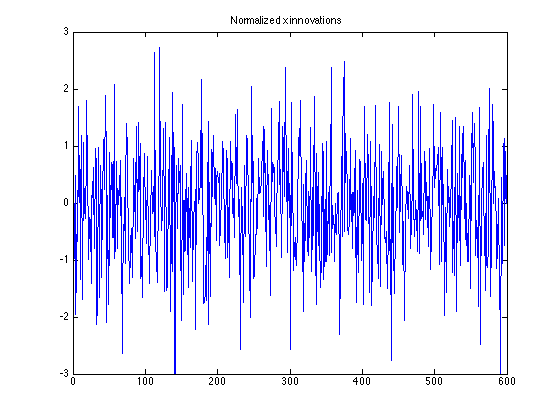
\includegraphics[scale=.4]{target_2_x_inno_q_0.png}
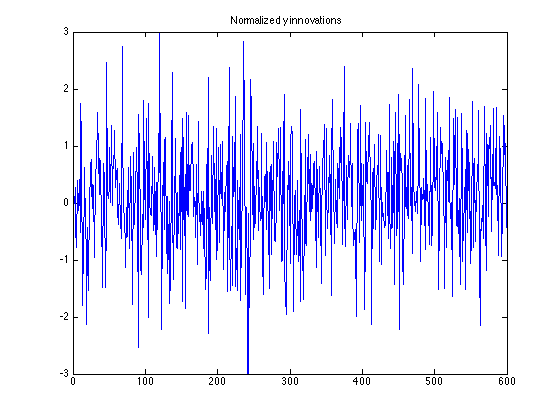
\includegraphics[scale=.4]{target_2_y_inno_q_0.png} \\

\paragraph{2.1.4 } The Percentage of x and y innovations that are less than 0 is $[ 52.50\%, 45.83\% ]$ \\

The plot of the running percentage of the x and y innovations that are less than zero : \\
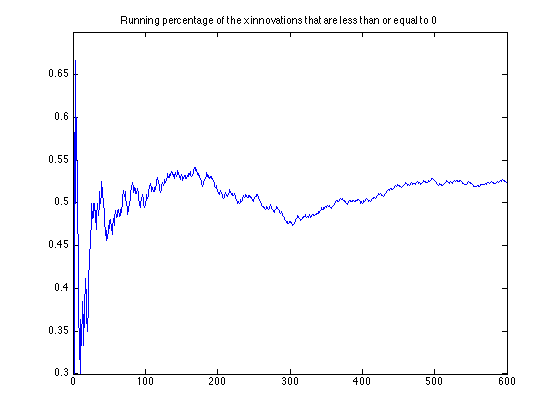
\includegraphics[scale=.4]{target_2_x_running_q_0.png}
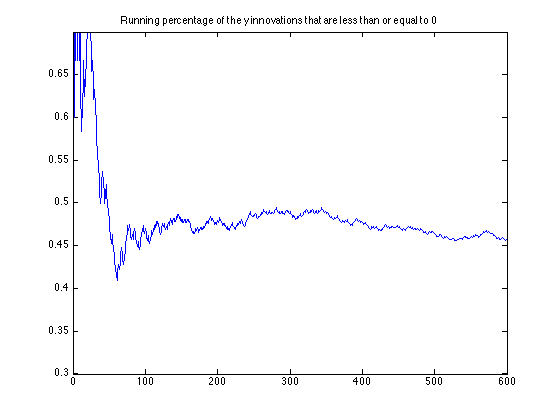
\includegraphics[scale=.4]{target_2_y_running_q_0.png} \\

In general, if a target doesn't follow constant velocity model and we let the filter run without adding $Q$ to the state estimate covariance before combining new information, the correlated bias due to the changes in time will be added and this often reflects in the normalized innovations graph. In our case the target motion has only slight deviation from true constant velocity which makes it look a little bit unsatisfied but relatively hard to spot substantial differences by looking at the normalized innovations in $x$ and $y$ with the given population size. Nevertheless, the filter could on longer produce a reliable estimate as a result of the progression of time. \\

\paragraph{2.2 } Changing the value of $q$, $q=0.01$ \\

\paragraph{2.2.1 } The state of the target at the time of the final observation is : \\
\begin{align*}
\text{mean with standard deviation} = 
	\left(\begin{matrix}
   -441.592942 & , &      0.118147 \\
    249.801248 & , &      0.120096 \\
     -0.496002 & , &      0.001068 \\
      0.280022 & , &      0.001069
	\end{matrix}\right)
\end{align*}
\begin{align*}
x\_final = \begin{bmatrix}
   -441.592942 \\
    249.801248 \\
     -0.496002 \\
      0.280022 
	\end{bmatrix}
\end{align*}
\begin{align*}
P\_final = \begin{bmatrix}
    0.01395871  &   0.00502150  &   0.00001566  &   0.00000561 \\
    0.00502150  &   0.01442316  &   0.00000560  &   0.00001621 \\
    0.00001566  &   0.00000560  &   0.00000114  &   0.00000000 \\
    0.00000561  &   0.00001621  &   0.00000000  &   0.00000114 
	\end{bmatrix}
\end{align*} \\

\paragraph{2.2.2 } The prediction of the state of the target one hour after the time of the final observation $(t=947.164131767)$ : \\
\begin{align*}
x(4547.164132) = \begin{bmatrix}
  -2227.201847 \\ 
   1257.879171 \\
     -0.496002 \\
      0.280022
	\end{bmatrix}
\end{align*}
\begin{align*}
P(4547.164132) = \begin{bmatrix}
   18.51007245  &   0.09379966  &   0.00412214  &   0.00001906 \\
    0.09379966  &  18.54540177  &   0.00001905  &   0.00413128 \\
    0.00412214  &   0.00001905  &   0.00000114  &   0.00000000 \\
    0.00001906  &   0.00413128  &   0.00000000  &   0.00000114
	\end{bmatrix}
\end{align*} \\

\paragraph{2.2.3 } The plots of the sequence of normalized x and y innovations separately : \\
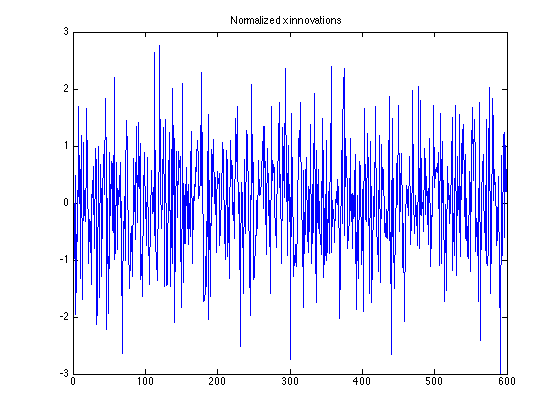
\includegraphics[scale=.4]{target_2_x_inno_q_0_1.png}
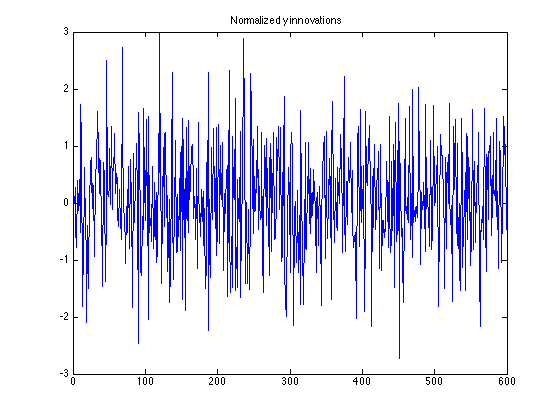
\includegraphics[scale=.4]{target_2_y_inno_q_0_1.png} \\

\paragraph{2.2.4 } The Percentage of x and y innovations that are less than 0 is $[ 49.67\%, 49.33\% ]$ \\

The plot of the running percentage of the x and y innovations that are less than zero : \\
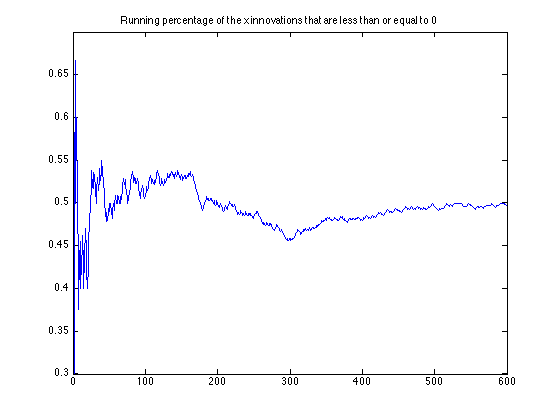
\includegraphics[scale=.4]{target_2_x_running_q_0_1.png}
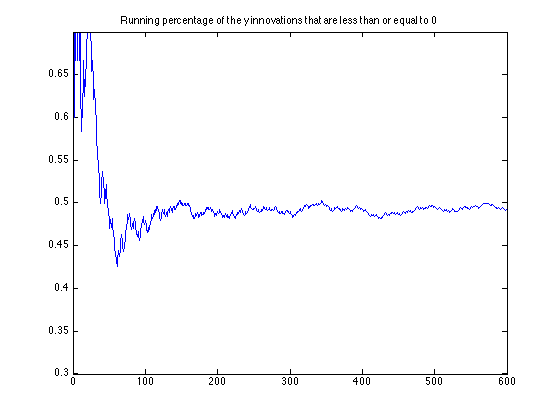
\includegraphics[scale=.4]{target_2_y_running_q_0_1.png} \\

As you have noticed covariance $P$ is getting more conservative to ensure that the estimate is consistent especially when we are trying to predict the state of the target far into the future. \\

For selecting the appropriate $q$ the filter has been executed many times with different values of $q$; and for the purpose of demonstration, below is the normalized innovations graphs for both $x$ and $y$ when setting $q=1$ and their running percentages of the innovations that are less than zero: \\

\paragraph{2.2.5 } The plots of the sequence of normalized x and y innovations separately : \\
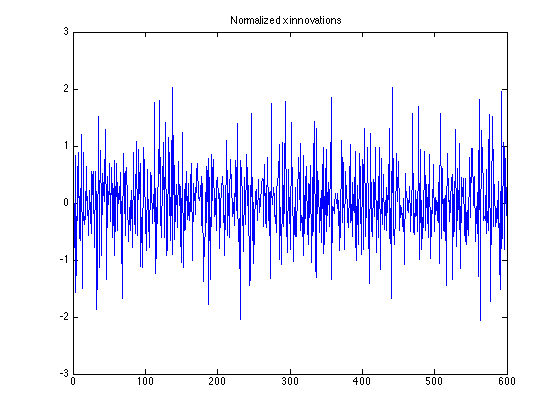
\includegraphics[scale=.4]{target_2_x_inno_q_1.png}
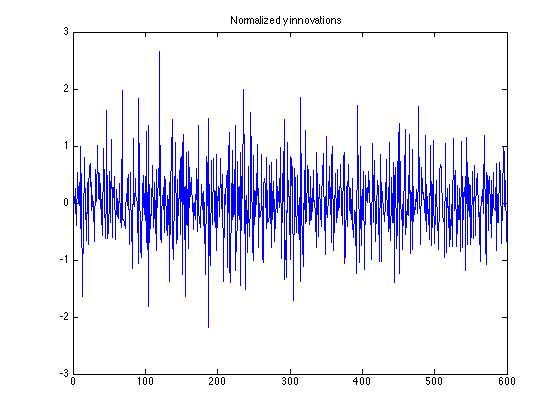
\includegraphics[scale=.4]{target_2_y_inno_q_1.png} \\

\paragraph{2.2.6 } The Percentage of x and y innovations that are less than 0 is $[ 50.50\%, 50.33\% ]$ \\

The plot of the running percentage of the x and y innovations that are less than zero : \\
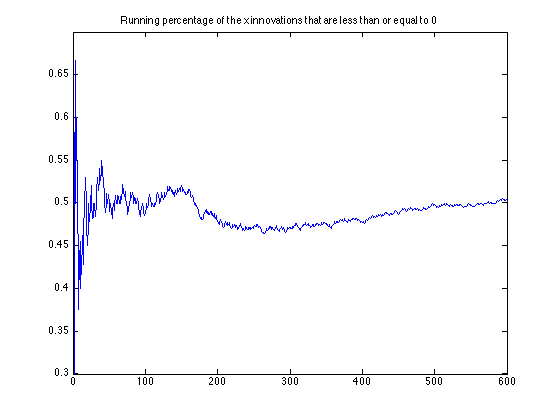
\includegraphics[scale=.4]{target_2_x_running_q_1.png}
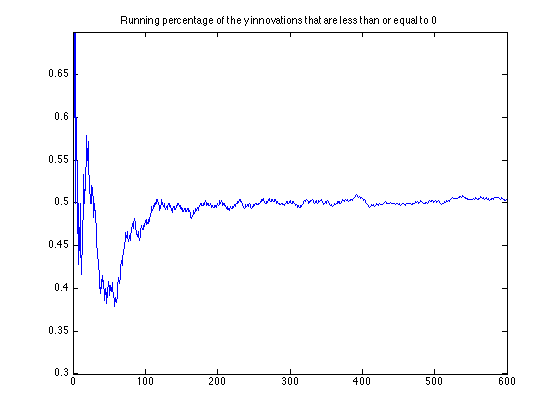
\includegraphics[scale=.4]{target_2_y_running_q_1.png} \\

\paragraph{Conclusion: } The bigger the $q$ applied to the filter the more conservative the state estimate will be. Ones will need to balance the value of $q$ not only to ensure consistent outcome but also to maintain adequate amount of the information retained. \\

\noindent And $q=0.01$ here can be considered as one of the best settings for the filter to produce consistent estimates balanced with information weight. \\

\newpage
\subsection*{Appendix:}
\lstinputlisting[language=Matlab, title=\lstname, basicstyle=\footnotesize]{assignment_7.m}
\lstinputlisting[language=Matlab, title=\lstname, basicstyle=\footnotesize]{filter_7.m}
\lstinputlisting[language=Matlab, title=\lstname, basicstyle=\footnotesize]{get_observation.m}
\lstinputlisting[language=Matlab, title=\lstname, basicstyle=\footnotesize]{predict.m}
\lstinputlisting[language=Matlab, title=\lstname, basicstyle=\footnotesize]{update.m}
\lstinputlisting[language=Matlab, title=\lstname, basicstyle=\footnotesize]{report.m}

\end{document}